
% LaTeX template document 
% Samuel Regandell 2003,2004
% Lines after '%' are commented out. '\' begins a command. 
% [...] indicate optional parameters. {...} indicate mandatory parameters.


% ============================================================================================= Preamble

%----------------------------------------- class of document
% documentclass[option,option, ...]{class}
% classes: article (for scientific reports/docs/invitations etc OBS-no chapters!)
%          report  (longer reports w.everal chapters/small books/PhD theses)
%          book    (real books)
%          slides  (for slides-with big letters/better use FoilTeX)

% options: 10pt,11pt,12pt                  (size of main font - default is 10pt)
%          draft                           (marks ``ugly'' typesetting results with black lines)
%          a4paper,letterpaper,a5paper etc (papersize - default is letterpaper)
%          fleqn                           (formulae is left-alligned, not centered)
%          leqno                           (formulae numbers on left, not right)
%          titlepage,notitlepage           (title on separate page or not)
%          onecolumn,twocolumn             (one- or two-column document)
%          landscape                       (changes page orientation)
%          openright,openany               (if next chapter will begin only on right-hand sides or not -
%  				            defaults differently in book and report; not available in article)							   
\documentclass[a4paper,12pt,notitlepage,twocolumn]{article}

% ---------------------------------------- page & text settings

% pagestyle{style}     (hint: to change style in current page, use \thispagestyle{style} )
% styles:   plain      (page-nr in footer; default setting)   
%           headings   (chapter & page-nr in header, no footer)
%           empty      (header & footer empty)

 \pagestyle{empty}

% linespread{factor} 
% factors:  1          (default line spacing)
%           1.3        (1.5 line spacing)
%           1.6        (double line spacing)

% \linespread{1.3}

%----------------------------------------- packages to load

% (See http://www-sop.inria.fr/miaou/latex/styles-eng.html for other packages.)

% usepackage[options,options, ...]{package} (packages for inserting graphics,language support etc)   


% \usepackage[swedish]{babel} % (swedish language support)
% \usepackage[T1]{fontenc}    % (swedish letters)

 \usepackage{graphicx}       % (allows postscript pictures in text with \includegraphics{file})   
% \usepackage{amssymb}        % (adds particular binary math symbols
                              %  such as ``approx.equal to'' etc.)
 \usepackage{fullpage}       % (reduces horisontal margins)
% \usepackage{makedx}         % (indexing system, activate with *Preamble* command \makeindex)

% \usepackage[options]{hyperref} % (should be *last* among packages to load)
                                 % (Allows for the creation of hyperlinks
                                 %  for use with e.g. latex2html or ps2pdf.
                                 %  In text, use \href{URL}{Name} or \url{URL}.        				 
                                 %  http://www.tug.org/applications/hyperref/manual.html)

%----------------------------------------- files to include

% \includeonly{filename,filename,...}   % (limits the files to be inserted later-better typesetting)

% ---------------------------------------- hyphenation rules 

% hyphenation(Hy-phen-a-thion Samuel) % (defines how to hyphenate ``hyphenation'', while  
                                      %  *never* hyphenating ``samuel'' or ``Samuel'').                                % \hyphenation{word list}

% ---------------------------------------- self-defined macros/definitions

% \newcommand{\new_command_name}[nr_of_args]{command_sequence or text}    % (nr_of_args defaults to 0)
% \newenvironment{\new_env_name}[nr_of_args]{process_run_before_environment}{process_run_after_environment}


%\renewcommand{\caption}[1]{\caption{\tiny $1}}

% ---------------------------------------- title page setup

\title{Interplanetary}
\author{Griatch (www.griatch-art.deviantart.com)}   % (separate several authors with \and)
%\date{}   % (for no date, put date field blank)


% ============================================================================================= Document Begin
\begin{document}


% ---------------------------------------- create title,TOC etc 

%\maketitle                   % (document title - specified above - is placed here)
%\tableofcontents            % (document might have to be run two-three times to get TOC right.)
                             % (add '*' after section command to have it not appear in TOC)
%\listoffigures
%\listoftables

% --------------------------------------- main text -------------------------------------------

\section*{\center Interplanetary\\by Griatch \\
   {\small (www.griatch-art.deviantart.com)}\\ {\small v0.8, March 2014}}

\section{Introduction}
Interplanetary is a
space-combat game for two or more players. It simulates the physics of
space travel in two dimensions along the ecliptica of our solar
system. 
\\\\

The movement system is borrowed from the long out-of-print boardgame 
\emph{Triplanetary} by GDW (currently owned by Steve Jackson Games). No resources 
from the original is used in Interplanetary.

\section{Game components}
Playing Interplanetary requires a normal 6-sided die (d6). The game itself comes as three 
separate files which you are encouraged to print copies of. 
\label{sec:game_components}
\begin{itemize}
\item The \emph{The Interplanetary manual} is what you are currently reading. It
  contains all the rule details but you will likely not have to refer
  much to it once you've played a game or two. 
\item \emph{The solar system map} acts as the playing
  field for the game. Interplanetary is played by drawing ship 
  vectors on this hexagonal gridded map using normal pencils. Whereas
  you can laminate a copy of this map and use erasable grease pencils,
  we find it's easiest to just print out a few paper copies and draw
  directly on them. The map can easily, and usually cheaply, be printed
  to A3 size (or bigger with a commercial printer).
\item  \emph{The game-aid} folds into three parts and contains the ship
  manifest and all tables needed for play. Each player gets one of
  these for every ship they control.  
\end{itemize} 
Interplanetary does not use any counters. We find this makes it very portable and
easy to play on the move. It is also easy to pause and continue at a
later time. If you have problems with the map getting messy (this can
happen when there are many ships), consider using coloured pencils to
separate tracks. Other inventive suggestions are to experiment with counters or
by placing the map on a whiteboard and use small magnets to mark ships.   

\section{Start of Play}

Determine a \emph{Scenario} (See Section \ref{sec:game_scenarios}). This 
often means the players have to outfit their ships. The Play-aid
lists all ship components available. For a first game, one of the simpler starting 
scenarios are recommended, with one ship per player.
\\\\
Once Scenario and ships are prepared, roll d6 to determine which player goes
first. This becomes the "first player" for the first round. You might want to 
have some sort of marker to mark who is currently the "first player", since this
position will shift for every turn. 

\section{Sequence of play}
\label{sec:sequence_of_play}
The game is played in \emph{rounds}, each round representing several days of 
real time. A round lasts from the "first player" and all around the table. When it 
would be the "first player"'s turn again, the round ends. 

One player is the "first player" and starts the round. Play continues
clockwise around the table. Once the round is over
(each player has completed their turn), the position of "first player" rotates
clockwise (meaning that the previously first player now becomes the last 
one to make their turn). The next round begins with the new "first player" taking
their turn. 
\\\\
During their turn, each player completes all the following steps, some
of which are optional. 
\begin{enumerate}
\item \emph{Launch phase}: Optional. Weapons that require time to reach their
  target (such as mines and missiles) are launched but don't actually move yet. Tick off 
  spent ammunitions on the game aid. Launched weapons inherit the old 
  vector of their launching ship plus eventual adjustments
  they are themselves capable of.  
\item \emph{Astrogation phase}: Mandatory. The ship and weapons launched now or earlier moves along its vectors. 
  If the player decides to burn fuel, the ship's vector direction can be changed. Launched weapons inherit the old vector
  from their launching ship plus eventual adjustments they are themselves capable of. 
  Tick off spent fuel on the game aid. If launched weapons hit something, or the ship passes into an
  enemy launched weapon, damage is decided by die rolls.
\item \emph{Gun fire phase}: Optional. The ship's mounted weapons (guns, lasers)
  fire against a target, taking into respect distance and
  relative velocities. Hits are decided by die roll. Targeted ships with suitable
  guns of their own may retaliate directly if they are not disabled or destroyed 
  by the initial attack.
\item \emph{Resupply phase}: Ships capable to do so may refuel,
  load/unload cargo and other actions which might be determined by the
  scenario.
\end{enumerate}

Below, each of these phases are described in more detail.

\section{Launching phase}

During this phase weapons such as missiles and mines are fired. This
happens before the ship actually moves in the turn.  Launched weapons 
``inherit'' the velcity vector of their launching spaceship and their
movements are plotted like a separate entity, taking gravity into
account. It can be a good idea to plot launched weapons with dotted
lines or different colours in order to separate them from spaceships.

Certain launched weapons may optionally apply thrust during launch. 
\\\\
A ship may only fire one launched weapon per turn.

\section{Astrogation phase}

During this phase the ship's movement is planned out and the ship
and all launched weapons belonging to the ship moves through space.

\subsection{Basic movement}

\label{sec:astrogation}
Interplanetary simulates Newtonian movement in two dimensions. Each ship
has an intrinsic velocity represented by a straight-line arrow (this
is called a \emph{vector}). The arrow has its tail at the location the
ship has at the beginning of the turn and points to the location it will
be at the end of the turn. A vector is always drawn between the
\emph{centers} of hexes. The basic rule of movement is: 
\begin{quotation}\noindent \emph{Any ship or other object not
        accelerated by thrust or gravity will move as it did on the
        previous turn and in the same direction.\footnote{Rewritten in another
          way this is also known as Newton's first law.}}
\end{quotation}

By burning a point of fuel, a ship can shift the endpoint of its
vector by one hex in any direction. A ship may only burn one unit of
fuel per turn. A ship with zero speed is marked with a simple dot on the map.

\begin{figure}[h!]\centering  
  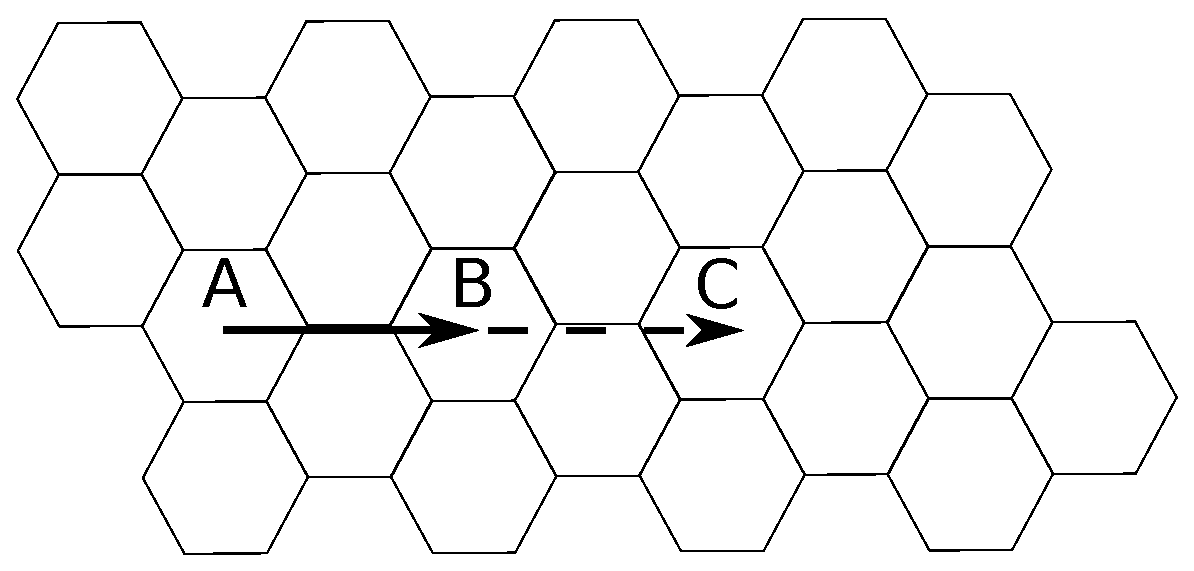
\includegraphics[width=0.5 \textwidth]{data/move_1.eps}  
  \caption{\footnotesize A ship moved from A to B in turn 1 will continue to C in
    the next turn if it does not accelerate due to gravity or burning
    fuel.}
\label{fig:1}
\end{figure}
\begin{figure}[h!]\centering  
  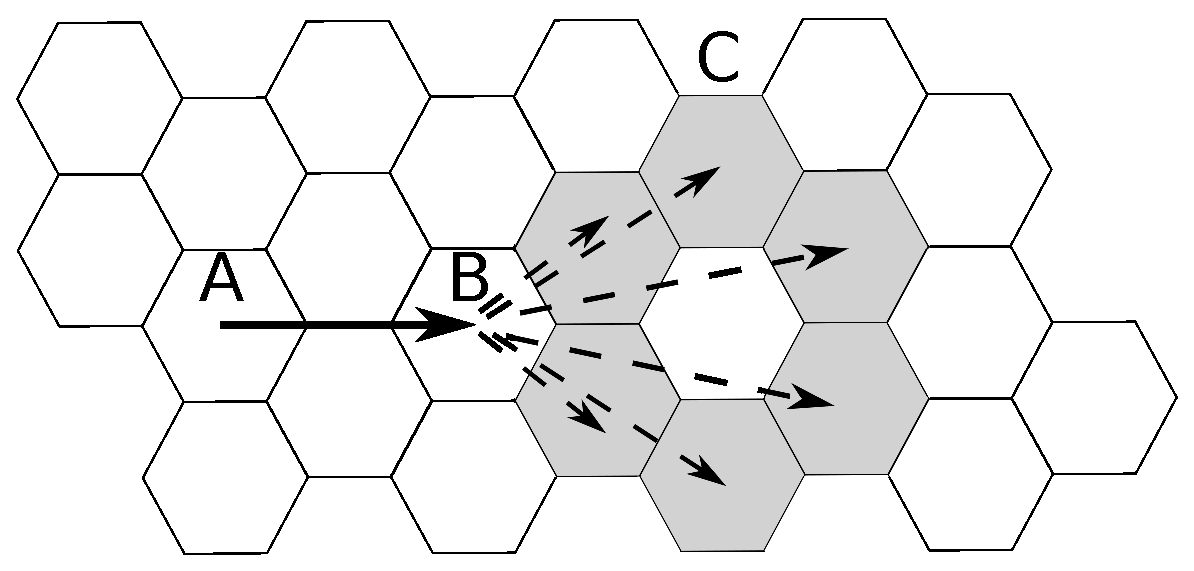
\includegraphics[width=0.5 \textwidth]{data/move_2.eps}  
  \caption{\footnotesize By burning one unit of fuel a ship may change
    the future tip of the vector by
    one hex.}
\label{fig:2}
\end{figure}
\begin{figure}[h!]\centering  
  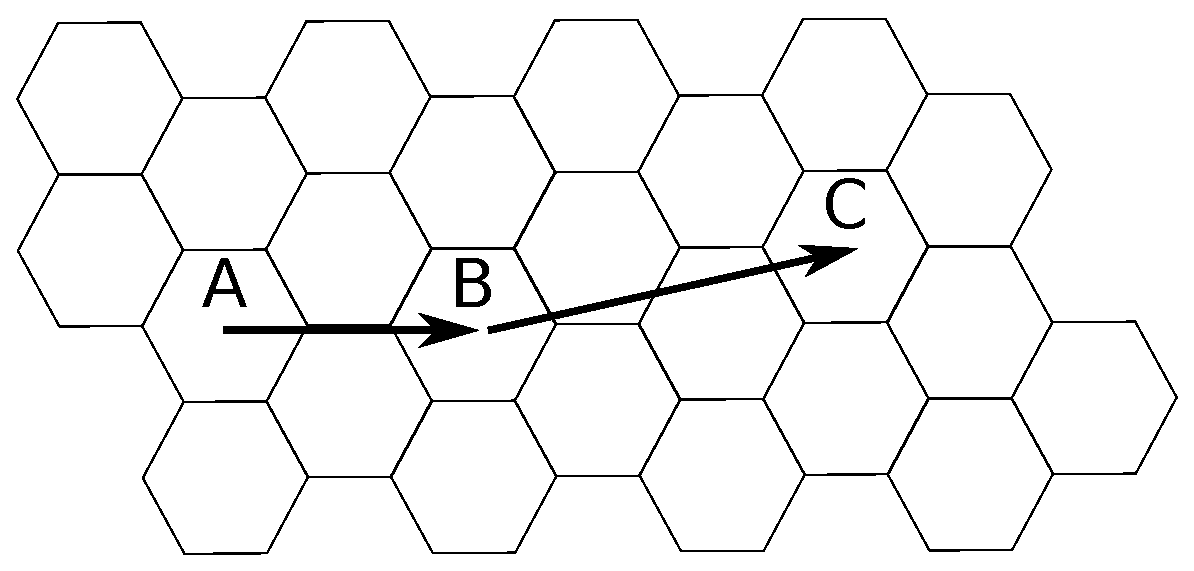
\includegraphics[width=0.5 \textwidth]{data/move_3.eps}  
  \caption{\footnotesize Here is the ship's final vector after having burnt fuel to
    change the vector to the ``north-eastern'' shaded hex in Figure \ref{fig:2}.}
\label{fig:3}
\end{figure}

\subsection{Gravity}

Stars and planetary bodies affect their surroundings through
gravity. Gravity is marked on the map as hexes with different types of 
arrows. On the turn \emph{after} a ship (or missile, mine etc) enters or passes through a gravity
hex, its vector is adjusted one hex in the direction of the arrow.  Several gravity hexes
can affect the vector each turn, the arrows are then just applied in
sequence. 

\begin{figure}[h!]\centering  
  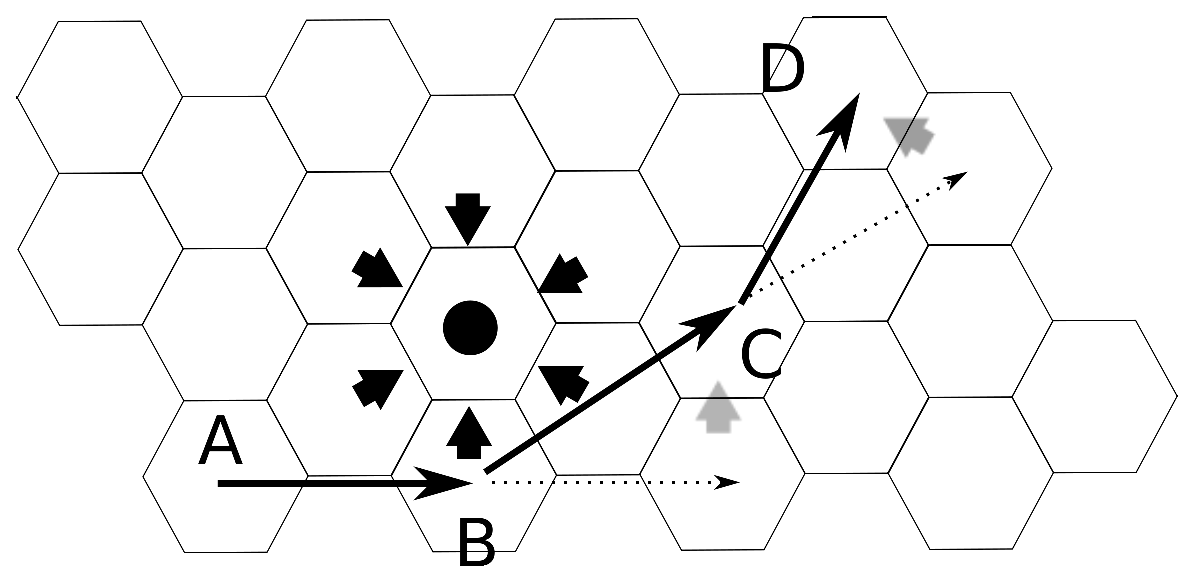
\includegraphics[width=0.5 \textwidth]{data/move_4.eps}  
  \caption{\footnotesize \emph{Effect of gravity}. Ship moves from A to B as normal, entering a
    gravity hex. 
    On the turn after (B to C), the vector's tip changes one hex
    in the direction of the gravity hex it passed on the turn
    before. Note that this new vector now also passes through a gravity
    hex. On the last turn, from C to D, the hex from previous turn adjusts
    the vector again. In this example the ship does not burn fuel, but
    if it did it would apply it after gravity corrections have been
    made each turn.}
\label{fig:4}
\end{figure}
\begin{figure}[h!]\centering  
  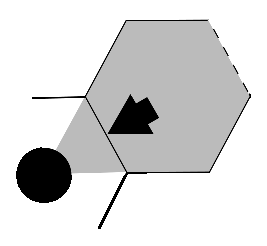
\includegraphics[width=0.10 \textwidth]{data/move_6.eps}  
  \caption{\footnotesize Ships passing between a gravity arrow and the gravitating
    object are affected by the gravity of the hex above. A
    ship passing exactly along the edge of a gravity hex is assumed to be
  affected by it \emph{except} if the edge is \emph{opposite} to the arrow. 
  If a ship should happen to travel along a valid edge between two
  gravitational hexes, the arrow \emph{closest} to that edge is used.} 
\label{fig:6}
\end{figure}

\begin{figure}[h!]\centering  
  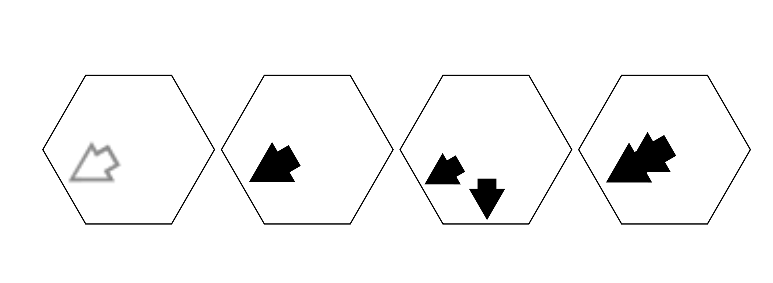
\includegraphics[width=0.5 \textwidth]{data/move_8.eps}  
  \caption{\footnotesize \emph{Gravity types}. From left to right: Weak gravity, normal gravity,
    two-directed gravity (choose which direction to apply) and double gravity.}
\label{fig:8}
\end{figure}

Apart from the normal solid black gravity hex described above, there
are three more types. 

\begin{itemize}
\item \emph{Weak gravity} is found around smaller moons and is marked with
  hollow arrows. If a ship enters a weak gravity hex, the player may
  \emph{choose} to apply that arrow or not. If not the hex is treated as
  empty space. However, if two weak gravity hexes are entered
  consecutively, the second hex's arrow entered \emph{must} be
  applied, regardless of what was chosen for the first arrow.

\item \emph{Two-directed gravity} are two arrows pointing in different
  directions in the same hex. These work like normal
  gravity, except the player must choose one (and one only) of the two
  arrows to apply.

\item  \emph{Double gravity}, marked by two overlying arrows, is found only
  around very heavy gravitational the Sun and shifts the tip of the vector two hexes in the
  direction of the arrow instead of just one.
\end{itemize}
\begin{figure}[h!]\centering  
  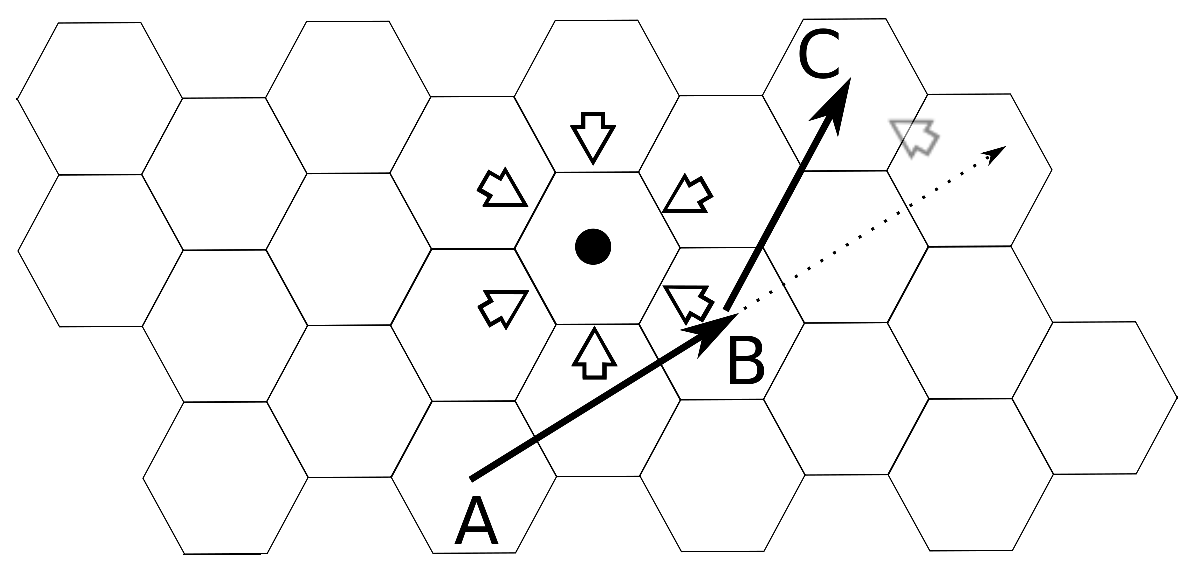
\includegraphics[width=0.5 \textwidth]{data/move_7.eps}  
  \caption{\footnotesize \emph{Weak gravity}. When passing through two weak gravity hexes, the second one
  to be entered always apply regardless of how the first one is
  treated (in this example the player chose to ignore the first hex,
  or point C would also have been shifted one hex upwards).}
\label{fig:7}
\end{figure}

\subsection{Entering Orbit}

Interplanetary allows for entering orbit around planets just using the normal
movement rules. This is done by entering orbit with a speed of
one, then burning fuel to break. You will then find you are orbiting
indefinitely without using any more fuel. The first turn the ship circles
without having to burn fuel is considered its first turn ``in orbit''.
When in orbit the ship may dock with orbiting bases to refuel and restock.

\begin{figure}[h!]\centering  
  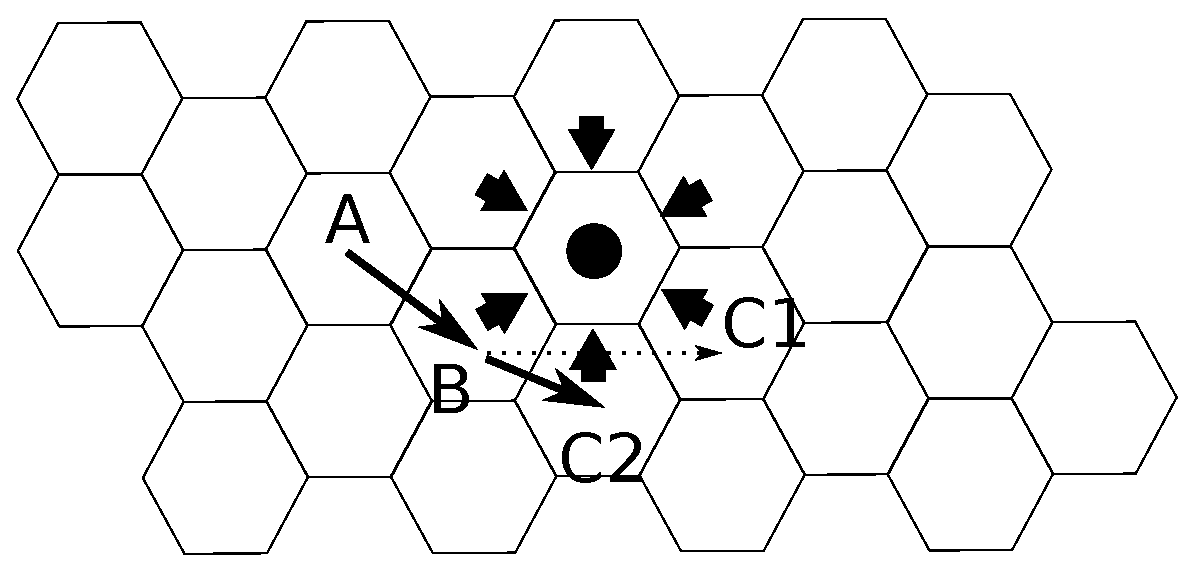
\includegraphics[width=0.5 \textwidth]{data/move_9.eps}  
  \caption{
\label{fig:9}\footnotesize \emph{Entering orbit.} Entering the vicinity of the
planet with speed 1 (A to B), the ship will on the next turn feel the effects of the
gravity arrow in hex B so as to try to accelerate it to point C1. If
the ship now burns fuel to break to C2 instad, it will find itsef in
orbit next turn, circling the planet without more use of fuel.} 
\end{figure}

\subsection{Planets}

A ship starting on a planet uses ground-supplied boosters to reach an
gravity hex above the planet's surface. This requires none of the ship's
own fuel. Once in orbit, the ship has zero speed and if it does not
spend fuel next turn it will crash back down onto the planet. 

A ship already in orbit may burn one fuel to land on the hex-side of the
planet it was above, assuming the game scenario allows it (like that
hex-side having a base or being friendly). When taking off again it
will do so from the same hex-side.  

If the vector of a ship intercepts the \emph{image} of a planet the ship is
assumed to have crashed and is destroyed.

\subsection{Asteroids}

A ship may only \emph{safely} pass an asteroid hex with a maximum
speed of 1. If passing at a greater speed, the player must roll
an ``Asteroid''-type Attack roll to determine eventual damage. Asteroid bases are 
also considered to be asteroid hexes in
this regard, but ships cannot accidentally crash into an asteroid base
the way they can crash into planets.  


\subsection{Other ships}

Each hex in Interplanetary represents a very large volume of space, so any
number of ships can coexist in a hex without any problems. 

\subsection{Bases}

Bases are found on asteroids, on planet surfaces and in orbit around
larger astronomical objects. They may be military installations or points of commerce. 
\\\\
Orbital bases are marked with little dots above planet surfaces. A ship \emph{in
  orbit} that passes over an orbital base may declare that they are 
  docking to it. Even though subsequent moves take the ship away from
  the dot, the ship is still considered docked. 

Planetary bases are also marked with small red dots. A ship \emph{in orbit}
may land by burning one unit of fuel while moving through the hex above 
the planet base. They will re-launch from that same hex-side.

Asteroid bases are visited simply by coming to a stop in the asteroid base's hex.
\\\\
Ships landed in a planetary base or docked to an asteroid station are
considered safe from all enemy attacks. A ship in orbit is still vulnerable to 
enemy weaponry regardless of docking status.

\subsection{Leaving the map}

Leaving the map usually means the ship is eliminated from play. If
players agree beforehand one can instead allow for the ship to reappear at the
point of exit after an agreed number of penalty turns. It would return
with a speed of zero.  

\subsection{Missile movement and attack}
\label{sec:missile_movement_and_attack}

Missiles move like space ships with very limited thrust capabilities. 
In order for the missile to be able to attack an enemy
\emph{the point of the weapon vector must enter the same hex as the enemy ship.}

The missile may also attack ships stopping in the same hex as the missile
on their own movement turns -- if so, the attack happens directly
at the end of that player's movement phase. 
\\\\
A missile attack is always \emph{optional} - the firing player decides if a capable 
missile attacks a target or not. If there are multiple targets in the same hex, the player 
must decide which one to attack. The missile is always lost in the attack, regardless
of the result.  
Missiles can also attack other missiles and the \emph{points} of Mine screens. Roll
an Attack roll as normal -- if the result is anything but a miss, the enemy weapon is
destroyed. Weapon-weapon attacks are always resolved before the attacked weapon has a chance to 
perform their attacks in the turn.  

\subsection{Mine and buckyball movement and attack}
\label{sec:mine_screen_movement_and_attack}
Mine screens are probes dispersing explosive mines in their
wake. They have no thrust capabilities of their own. They are less
destructive than missiles but are easier to hit with. Mine screens
will "attack" \emph{everything intercepting or passing through any
part of their current vector}. The mine field is not lost in an attack,
it will continue to attack targets until its time runs out (after 5 turns). 

"Buckyballs" are unguided kinetic projectiles dispersed in a large shroud.
They are completely unguided and their damage is determined by the relative
velocity with which it hits its target. Buckyballs, like mines, will attack
everything intercepting or passing through any part of their current vector, 
but unlike mines they will be consumed if their attack is successful. If 
not successful, the buckyballs will keep going and attack the next target it 
hits. 

A mine screen or buckyball shroud will also attack a ship passing  through the mine vector on its own turn -- if so,
the attack happens at the end of that player's movement phase. 

\begin{figure}[h!]\centering 
  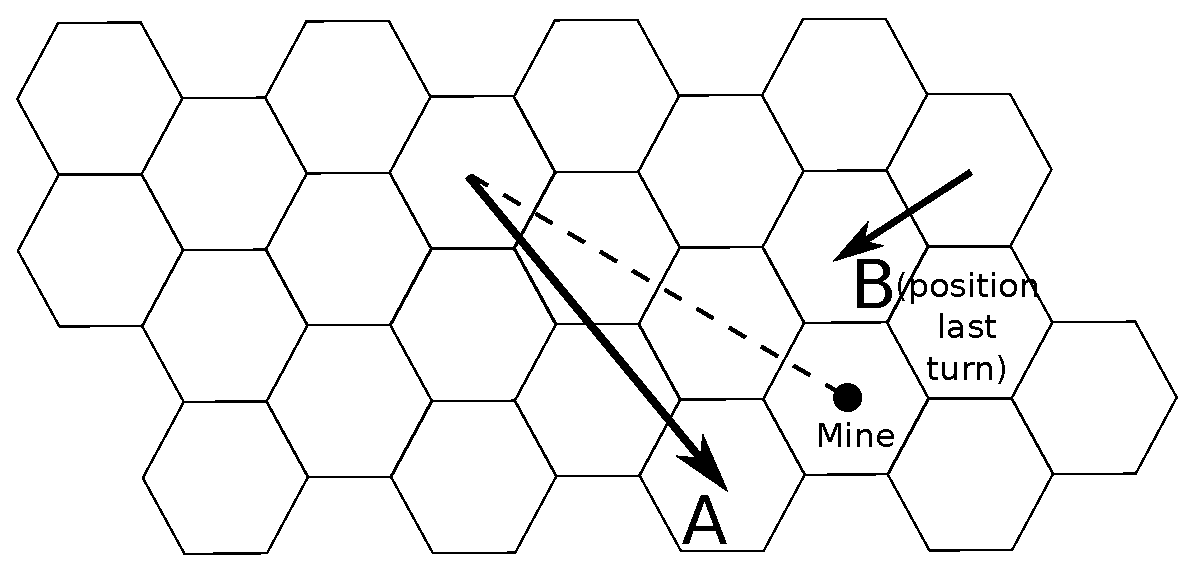
\includegraphics[width=0.5 \textwidth]{data/combat_1.eps}
  \caption{\footnotesize \emph{Use of mines}. In this turn,
    ship A drops a Mine (and boosts to the side to avoid 
    running into it itself). When it's B's turn, ship B will
    intersect the Mine's vector (and thus be hit) unless ship B
    changes its course. The mine field will stay in space for 
    another four turns.}
\label{fig:10}
\end{figure}

Mine and Buckyball attacks are \emph{not optional} -- they will attack everything,
including the ship launching them. This means the firing ship must
veer to the side after firing in order to not run into its own ordinance.


\section{Gun phase}

The ship's guns can fire once every turn. Guns are assumed to have infinite ammunition
and to hit immediately. 
\begin{figure}[h!]\centering 
  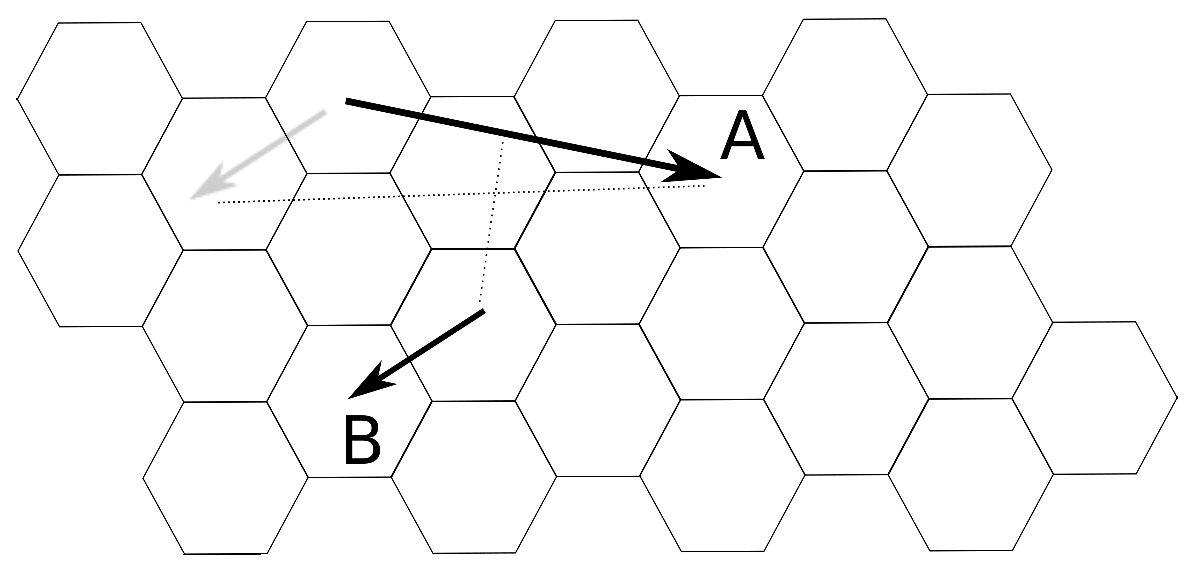
\includegraphics[width=0.5 \textwidth]{data/combat_2.eps}
  \caption{\footnotesize \emph{Calculating gun attack modifier}. Ship A fires
    on B. The distance
    between the ships are calculated at the closest point of their
    vectors to be 1 (which is less than 2 and thus ignored). The relative velocity is much bigger; by vector
    addition it is found to be 4, which is two bigger than 2. The
    attack roll is thus made with a -2 modification. } 
\label{fig:11}
\end{figure}

Guns are affected by the \emph{distance} to the target as well as its
\emph{relative velocity}. The distance is counted from 
the \emph{closest} point of contact between the two ships'
vectors (the guns are assumed to fire at the optimal point). For every hex of 
distance \emph{greater than 2}, a -1 modififier
is applied to the attack roll. The relative velocity is found by
simple vector subtraction (shift one vector's base to the base of the
other and count the hexes between their arrowheads). Again, any
relative velocity greater than 2 adds a -1 modifier. 

Most ships with guns also have \emph{retaliation
  capability}\footnote{This represents the fact that firing the guns in 
  itself shows where you are}. In game terms this means that 
  once the attacking ship has rolled its attack and all eventual damage been applied, 
  the attacked ship may fire back with its own guns (assuming its guns 
  allow it and the ship was not disabled or destroyed in the initial attack).   

\section{Resupply phase}

In order to re-supply during play, the ship must be docked to a space
station, asteroid base or planetary installation. 
\\\\
When docked with or landed at a base, the player may buy fuel and
restock weapons assuming the scenario allows it. Available payloads and costs
can be found on the play-aid. See also Section \ref{sec:payload} for more
detailed descriptions.

\section{The attack roll}
\label{sec:attack_roll}

An \emph{Attack roll} is done whenever a gun is fired or a 
launched weapon gets in a position to strike.

The weapon type determines which Attack table to use, see the game aid. The
attacker rolls d6 and applies and modifications required to it. Such modifications
could be weapon bonuses, effects of distance and velocity, as well as 
eventual defenses of the enemy. 

The result is either a miss, a hit or a "Disabled" result (or a combination of 
the two). 

All ships react the same way to damage\footnote{With the 
weight-limitations inherent in any realistic spaceship design it is
impossible to add enough armour to match the cheap and terrible destruction
capabilities of space weaponry. If a tactical nuke detonates at point blank
range it doesn't really matter if you are a large battleship or a small frigate
-- the only difference is how large the scraps will be...}. The weapon
effects are listed as follows on the play-aid: 

\begin{itemize}
\item Disabled. The ship's Engine 
  and its Reactor are temporarily offline. The ship cannot burn
  any fuel while being disabled. It also can normally not fire any
  guns (but it can however still use launchable weapons). When a 
  ship is disabled by gun fire it cannot retaliate. 

  Disabled results do \emph{not} stack. Another Disabled results applied
  to an already disabled ship is simply ignored\footnote{For realism, assume
  the ship is running dark, making it harder to hit}. A disabled
  ship is still affected by all other types of damage.
\item A hit. Roll d6 to decide which
  ship subsystem was hit. For each of these hits, roll d6 again to see
  how much damage was applied to that subsystem. See Section
  \ref{sec:ship_subsystems} for more information about the subsystems
  and about how damage is assigned to them. 
\end{itemize}

\subsection{Ship subsystems}
\label{sec:ship_subsystems}

The play aid has a central image of a spaceship surrounded by
numbers in a hexagon shape. Each of the six locations around the
ship represents a certain ship subsystem. Each subsystem can hold one
or more ship \emph{modules}.

On the play-aid, squares indicate module mount points whereas circles 
show how many points of damage that component can withstand before failing. 
When your ship get a hit as described in Section \ref{sec:attack_roll}, 
roll a die to determine which subsystem was hit. Roll again to determine 
how much damage is applied to that subsystem. 
\\\\
The player receiving the damage may distribute the damage points as 
they see fit between the modules of the subsystem, including checking
damage circles in slots not holding any modules (these can be considered armour). 
Modules will function perfectly as long as they have at least one unchecked damage circle.
\\\\
Once all the damage circles of a subsystem has been filled, that subsystem
cannot absorb any more damage. Further damage will be applied to the \emph{Structure}
subsystem. When \emph{Structure} is destroyed, so is the ship.

\begin{itemize}
\item \emph{Structure} (hit location 1) represents the basic structure of the
  ship, its command modules, computers and other vital systems. The
  Structure subsystem has 8 hit points (represented by circles); when
  all are gone the ship is destroyed. Whenever another subsystem receives 
  more damage than it can hold, the excess damage is applied to Structure. 
\item \emph{Gun Mounts} (hit location 2) holds the Guns of the the ship.
  It can take 6 points of damage before the guns are destroyed. 
\item \emph{Launchers} (hit location 3) is the mounts and bays for all launched ordinance. 
Six weapons may be mounted, each representing one point of damage. The mounts are numbered
from 1 to 3 on the play aid.
\item \emph{Fuel/Engine} (hit location 4) represents the fuel tanks and
engine block of the ship. As the ships accelerates, fuel is spent by ticking off
  the squares here. The amount of damage this subsystem can take is equal to the number 
  of units of fuel remaining (as fuel is spent, tanks go empty and offers less buffer against
  damage). All damage applied to this subsystem means a loss of fuel. 
\item \emph{Reactor} (hit location 5) This is the auxiliary power core of the ship. It must work
in order for Systems to operate. It can take 6 damage before breaking down. 
\item \emph{Systems} (hit location 6) represents all support structures and special
additions to the ship, like computers, sensors and various armor expansions. Systems usually
add various bonuses to ship operations. They require a working Reactor in order to 
operate. Two System modules may be installed, each able to withstand 3 points of damage. 
The two mount points are marked 1 and 2 on the play aid.
\item \emph{Single Use} These are single-use additions to the ship such as expendable
boosters and other items. They cannot be damaged by a roll but may be sacrificed: Doing so 
will absorb one unit of damage instead of another subsystem. A maximum of two 
single-use modules may be mounted. 
\end{itemize}


%\section{Payload}
%\label{sec:payload}
%
%This constitues a brief technical description of the various 
%payloads available. They are usually bought at the beginning of play,
%but may also be added by landing or docking at a base during the game. 
%Each payload module is listed with a credit cost and a mass. How many credits each
%player has available is decided upon before starting play. The mass of
%all the payload, including fuel, must never exceed the ship's \emph{Max total mass} attribute. 
%
%See the play-aid for the exact numbers and costs for each item.
%
%\subsection{Fuel}
%
%Fuel is the life blood of any spaceship. A ship cannot carry more fuel than 
%allowed by its \emph{Max Fuel} property (the size of its tanks). A ship can 
%only burn one unit of fuel per
%turn to change its velocity. A ship can opt to carry less fuel than
%the maximum, e.g. in order to fit additional modules. 
%
%\subsection{Systems}
%
%These are collections of support systems that improve the ship in
%various ways. Unless noted otherwise, Systems only work if the Reactor
%is operational. System effects do not stack (so there is no point in
%adding more of the same type).
%
%\begin{itemize}
%\item \emph{Repair AI} - A centralized robotic workshop and miniature
%workforce. The system allows the slow repair of damaged subsystems. One 
%point of damage will be repaired every 5 turns (counting from the moment the 
%first point of damage is received). The repair system will not replace Fuel lost
%due to damaged fuel tanks. Requires a working Reactor 
%\item \emph{Armour AI} - The Armour AI uses minute ship movements to redirect damage from 
%vital sytems. If the \emph{Reactor} or \emph{Structure} subsystems are hit, the Armour AI allows
%the re-routing of 1 point of damage to any other subsystem the player chooses. Requires 
%a working Reactor.
%\item \emph{Fuel Scoop} - An electromagnetic funnel for collecting gasseous hydrogen
%from either the Sun or Jupiter. In order to use the Fuel Scoop the ship must pass \emph{inside or 
%on the edge of} the hex of the respective astronomical body (i.e. through the thin white area
%just next to the Jupiter/Sun image on the map). The scoop will immediately refuel d6 units 
%of fuel to the ship. The Scoop requires a working Reactor to operate.
%\item \emph{Capacitators} - The capacitor activates when a ship becomes disabled. It
%allows the ship guns to \emph{retaliate} for 2 additional rounds after being disabled. 
%This includes retaliation to the attack in which it became disabled. The ship can only retaliate 
%if its guns actually has that capability. 
%\item \emph{Large Capacitors} - a larger version of the Capacitor. This system activates 
%when a ship becomes disabled. It allows the ship to retain normal
%weapon capabilities for 2 rounds after being disabled. 
%\item \emph{Battery pack} - chemical energy store kept charged by the Reactor. If the
%Reactor is disabled, the Battery Pack keeps the ship (Guns and Systems) operational for another
%5 rounds. The battery pack is thus an exception to the rule that System modules requires a working Reactor
%to operate. If the Reactor comes back online (even if only temporary), the Battery pack 
%is immediately fully recharged. 
%\end{itemize}
%
%\subsection{Single Use}
%
%These modules can all only be used once. A ship may carry two single-use modules at
%a time. Single-use modules can be used also if the ship is currently disabled.
%
%\begin{itemize}
%\item \emph{Chemical booster}. This is a pack of rockets with solid
%  propellant, pretty much like huge firework-rockets that are ejected
%  once they burn out. Chemical boosters supply 1 additional point of
%  thrust when used. This additional point does not consume any fuel (the rocket
%  holds its own fuel).
%\item \emph{Orion booster}. This powerful single-use system integrates a
%  deployable absorber plate with a nuclear charge of several kilotons. The
%  nuclear weapon is ejected just behind the spaceship and
%  detonated. The absorber plate protects the ship while converting the
%  energy of the blast into a powerful acceleration\footnote{This may
%    sound  bizarre, but a variant of this has been seriously
%    considered for a full ship drive.}. An Orion booster supply 2
%  additional points of thrust in the turn it is fired. It does not consume
%  any ship fuel.
%\item \emph{Spin booster}. This is an extra set of emergency rockets
%  used to rapidly rotate the ship on its axis in an emergency. It allows
%  for a last-minute re-distribution of damage over a larger area. If hit
%  with a Targeted hit, roll hit location as normal.  But before rolling
%  damage, declare using the Spin booster. The player may then
%  re-distribute the rolled damage as they please between all the ship's
%  subsystems.
%\item \emph{Evasive booster}. This emergency rocket pack allows for emergency
%  evasive actions. When used, increases the maximum "safe" speed to use when
%  passing an asteroid hex to 3. The booster is good for all asteroid hexes 
%  the ship passes through in the turn it's fired. The Evasive booster can also be used defensively 
%  to yield -2 to an enemy's Ramming attack.
%\item \emph{Randomizer boost}. This set of emergency rockets fires in a 
%  random sequence to make it harder for an incoming projectile to hit. Declare
%  use before enemy rolls for their Gun attack. Roll d6 and remove the result 
%  from the enemy's attack roll. This can be used also against retaliation
%  fire.
%\item \emph{Friction shield}. This is a shield mounted at the front
%  of the ship, specifically used for breaking using the atmospheric friction of Planets
%  and moons. The friction shield can not be used for Mercury, The Moon or Europa. 
%  The Friction shield yields +1 thrust, \emph{only} as part of a move that will leave 
%  the ship in a stable orbit next turn. This additional thrust does not expend
%  any fuel. The shield cannot be used to dock with asteroid bases. 
%\item \emph{Re-entry shield}. This shield uses atmospheric friction to to make
%  re-entry. It can not be used on the Sun, Mercury, The Moon or Europa. 
%  It can only be used if the ship moves with a maximum speed of 2 and allows a ship
%  colliding with a planet to land instead of being destroyed.
%\item \emph{Emergency patch pod}. This module instantly repairs 1 point of damage
%  to one damaged subsystem. It will not replace fuel lost due to damaged fuel tanks.
%\end{itemize}
%
%\subsection{Launchers}
%\label{sec:launchers}
%The Launcher subsystem is loaded with various launchable ordinance. Six launchable
%weapons can be loaded in the Launcher subsystem at one time. Since each weapon holds its own
%fuel and power, the launcher operates independently of the ship's Reactor. 
%
%\subsubsection{Mines}
%Mines move and attack using the rules in Section \ref{sec:mine_screen_movement_and_attack}.
%\begin{itemize}
%\item The \emph{Mine screen} is a small automated probe dispersing a vast
%  field of small unguided explosive charges and shrapnel around it.
%  Mines are not as destructive as other launched weapons but they are easier to hit
%  with. They make for powerful strategic weapons to restrict the movements of an enemy. 
%  
%\end{itemize}
%
%\subsubsection{Missiles}
%``Missiles'' is the collective name for powered deep-space weapon platforms. Missiles
%are small spaceships of their own. They carry their own fuel and sophisticated
%guidance systems and sensors. Missiles carry high-yield nuclear warheads, making
%them the single most powerful weapons in TriAv, delivering massive damage if they
%are able to get near their target. Missiles move and attack using the rules 
%in Section \ref{sec:missile_movement_and_attack}.
%\begin{itemize}
%\item \emph{Rockets} have only a small fuel supply, rockets may only apply
%  up to 1 point thrust at the moment of launching from the ship, after which it
%  will cruise until it enters the hex of an emeny or self-destructs. 
%\item \emph{EMP rockets} has the same chassis as
%  rockets but the warhead is replaced with a nuclear charge tuned
%  to release energies causing maximum harm to electrical
%  components. EMP rockets will not cause any direct damage to an enemy
%  but can disable them for a longer time than any other weapon type. It is thus
%  a powerful tactical weapon.
%\item \emph{Missiles} are bigger vehicles than rockets but work along the same
%  principles. Their bigger engine and fuel supply allow them up to 2
%  points of thrust at the moment they are launched from the ship. 
%\item \emph{Torpedos} are intelligent stealth weapons capable of being
%  dropped out of their launch tubes to drift through space until the
%  right time has come to fire its engine. A torpedo has one point of fuel 
%  to spend, but may apply that thrust at \emph{any time} during its
%  flight. 
%\item A \emph{Booster Torpedo} is a torpedo with extra fuel tanks. It
%  has two units of fuel and may apply thrust at any time during its flight
%  (it can only burn one unit per turn).
%\item A \emph{Target decoy} is a "fake" ship that mimics the heat emissions
%  and electronic signature of the parent ship. The decoy does not have any
%  thrust capabilities of its own. As long as the parent ship stays in the
%  \emph{same hex} as the decoy all enemy guns and missiles have -2 on their 
%  attack roll. The decoy will loose power after 5 rounds like any launched
%  object, but during this time it will work also if the parent ship leaves and 
%  then re-enters its hex. 
%\item The \emph{Kinetic Buster} is a tactical weapon, only usable against
%  planetary installations and orbital stations. The Kinetic Buster is a
%  massive, sleek bullet delievering enormous kinetic energy to a stationary
%  target. The Basekiller is unguided and must be launched with a speed
%  of at least 3 to deliver enough energy. No spaceships can be hit by the 
%  Kinetic buster. 
%
%  A Kinetic Buster hitting a planet hex side will destroy any base
%  located there. The attacking player can choose to destroy an orbital
%  base above that side instead of hitting the planet's hex below. A hit on an asteroid
%  base will destroy that base, converting its hex into a normal
%  asteroid hex. All ships docked or landed at attacked bases will
%  be destroyed along with the base, but not ships that happens to be
%  passing by in the same hex.
%
%\end{itemize}
%
%\subsection{Gun mounts}
%
%Spaceship guns are massive installations using a large amount of
%power. The gun mount subsystem can hold a maximum of two guns at any
%time. Both mounted guns can then fire independently at two targets or
%twice at the same target. All guns are also capable of retaliation
%fire. The gun mount subsystem requires a functioning Reactor to operate. 
%
%\begin{itemize}
%
%\item \emph{Railguns} use a catapult-like rail system to electromagnetically launch a
%  metallic slug at terrifying speeds. The projectile is just a dumb chunk of metal --
%  the kinetic energy released upon a direct hit is enough to punch
%  through anything. But even though
%  the slugs travel fast, even a minute course change by the enemy while the slug
%  travels will cause it to miss by hundreds of kilometers. 
%\item \emph{Heavy Rail cannons} does not fire
%  heavier projectiles than railguns, rather it has a much heavier
%  support structure that allows them to fire the slug with higher speed. A
%  shorter time of travel means higher precision and impact. A
%  heavy railgun gives +1 to the attack roll. The slower aim means that 
%  the gun may only perform one retaliation attack per round.  
%\item \emph{Laser batteries} use large capacitors to discharge a
%  powerful pencil-thin beam of X-ray radiation across
%  space. Delivering this energy to a point on the target quickly cooks
%  through any defenses. The stubby laser turret itself is not very
%  heavy, the problem is the massive energy requirements for each
%  shot. A laser battery \emph{ignores} any effects of relative
%  velocity on its attack roll.
%\item A \emph{Mass driver} is a electromagnetic railgun stretching the
%  full length of the ship. It is designed to launch a heavier sliver of
%  metal. Sometimes considered as a type of spaceship drive in itself,
%  the kinetic energy delivered by a massdriver slug is tremendeous. A
%  massdriver gives a +2 to the attack roll. Its structure however
%  makes it unsuitable for retaliation-fire. 
%\item \emph{Flak guns} are defensive weaponry. These automatic
%  guns fire shrapnel ammunition that fill the space around the
%  aircraft with small objects, expanding gas and pencils of laser light in order to
%  confuse missile sensors our destroy incoming mines. Every Flak
%  decoy gun reduces the attack roll of any launchable weapon by 1. 
%\end{itemize}

\section{Base services}

A base offers the following services:

\begin{itemize}
\item \emph{Refuel} Fuel fill up to max capacity. 
\item \emph{Refit} Bases allow to replace non-launched weapons, guns and system modules 
on a one-to-one basis, allowing the player to change their loadout as they see fit. 
\item \emph{Orbital repair}. Orbital space stations only. The shipyards of an orbital station
    may repair 1 unit of damage per round (in any system). 
\item \emph{Planetside repair}. The larger shipyards of Planet and Asteroid bases may repair
    2 units of damage per round (among any systems). 
\item \emph{Planetside launch}. Planet launch is considered free, using free boosters or
launch rail mechanisms (so no fuel will be spent). The launch place the ship in the hex
above the base with a speed of 0, so it will need to apply thrust next turn in order to not
crash back down. 
\end{itemize}


\section{Optional rules}
\label{sec:optional_rules}


\subsubsection*{Space rendevouz}

By matching vectors (speed and position), a ship may attempt to get
into physical contact with another ship.  Both ships must willingly
accept the space rendevouz for it to happen. Fuel and launched
weaponry (but not mounted weapons) may be exchanged between the two
ships. Both ships must skip a turn to
complete the move. 

This rule allows for refuelling tankers and other supply ships as well
as allies helping each other out. 

\subsubsection*{Surrender}

This allows for a Space rendevouz, as above, between enemy ships,
where one of the ships have surrendered to the other ship. The
conditions of the truce is agreed on beforehand by the players --
usually how much loot the winner is allowed to take from the defeated
ship, or how many Points should be transferred. A surrender is
considered a binding bargain for both sides. The surrendering ship may not fire
upon the approaching ship and whatever prize was promised will be
transferred as agreed. 

\subsubsection*{Boarding}

By matching vectors (speed and position) with a \emph{disabled} enemy ship, a ship may
attempt to launch a boarding party to subjugate it. Both players roll
a die; if the attacking player roll the highest, the enemy is
defeated, otherwise the defender has fought off the attack. Only one
boarding attempt can be made every turn, and \emph{only} if the
attacking ship is not performing any other attacks. It may also not
counterattack. 

If the enemy is defeated, the scenario may decide what happens; it
could be anything from being allowed to loot the enemy ship to the
attacking player now playing the enemy ship as their own. 

\subsubsection*{Civilian ships}

By defining some ships to be ``civilian'' one can define all sorts of
interesting scenarios. Civilian ships can carry weapons in their cargo
holds but cannot launch them. They can represent supply
ships or targets to raid if used with the Space rendevouz or Boarding
rules respectively. 

\subsubsection*{Special Asteroids}

The coloured asteroids around Clandestine are impassable unless you
know the exact route. Only ships belonging to the side that controls
Clandestine may enter these hexes, others are considered to have
crashed. Missiles entering a special asteroid hex detonates harmlessly
without affecting ships in that hex (ships \emph{already inside} such a hex can
however fire out. Cannons work both ways). 

\subsubsection*{Kinetic Buster}

A special Launched weapon is made available, the Kinetic buster. This
is a massive space-to-ground weapon intended to launch against bases
and installations. A ship can only carry one kinetic buster at a time.

When attacking, roll d6. If the roll is lower than the relative velocity
of the missile and its target, it will have destroyed its target. 

Example: A ship travelling with a speed of 5 launches a kinetic buster
at a planetary base. The relative velocity is 5 since the base is 
stationary. When hitting, the attacker must roll under 5 (1-4) to destroy the
target. 


\subsubsection*{Bases pick sides}

Bases can be assigned to a ``side'' and count some of the players as
enemies. All bases have a \emph{zone of control} with is marked with a
coloured outline on the map. Ships on the edge of such a zone is
considered to be inside the zone. It is impossible to dock and
refuel/restock at an enemy base unless this is especially defined in
the current game scenario. Bases act first of all on the
board\footnote{Meaning that ships tend to react to the actions of bases and
  not the other way around.}. 

Bases may have defences. A base can fire
a launched weapon of type \emph{Missile}(see Section
\ref{sec:payload}) every two turns, or as often as defined in the
scenario. The base is assumed to have an infinite amount of missiles. 
All weapons are affected normally by gravity. 

Bases are generally equipped with one (or more) \emph{Mass driver}
(Again, see Section \ref{sec:payload})
type guns. Bases may not fire its guns at ships outside its control
zone range.  

The only weapon capable of harming a base is if the Kinetic Buster rule
is used. 

\subsubsection*{Mine fields}

Mine fields may be deployed depending on the scenario. They consist
of stationary \emph{Mine} weapons located in space at the
beginning of play. They most often have zero speed. A mine in a mine
field use the same attack table as a launched Mine, but is not
destroyed after 5 turns but will last indefinitely (they are also 
not destroyed when hit).

\subsubsection*{Fog of war}

This is mostly suitable for campaign scenarios and simulate a lack of
knowledge about the enemy loadout. Players don't reveal their ship manifests to each
other. Launched weapons are announced and drawn openly when fired
and firing guns will reveal the gun type. 

Each ship has a detector range or 3 hexes, only when coming closer
than this from each other do the two detecting players show each other
their manifests.  In the case of bases belonging to a
particular side, a ship passing within their detector range will also
reveal the ship's manifest to all players on the base's side. 

Fog of war is mostly suitable for bigger scenarios. One can envision a
fleet masking their movements by deploying unarmed empty ships as
decoys. 


\section{Game scenarios}
\label{sec:game_scenarios}

These are some simple game scenarios for quickly getting going. There
is not much ``story'' to these; they are simply
fun setups for a quick game. One can easily invent more elaborate
scenarios and campaigns. 

\subsection{Training}

For getting to learn the movement and gravity rules, newbie players
may get going with the following initial scenario.

\subsubsection*{Setup}
Players start with unequipped ships. They start on Earth and are
assumed to launch with boosters into an orbital hex of their choice on
the first turn.   

\subsubsection*{Goal}

Goal is to enter at least one gravity hex around
Venus, Mercury and the Moon -- in that order. The winner is the first
one to return to proper orbit around Earth. 


\subsubsection*{Variations}

For full training in more aspects of the game, add a Artillery gun, a mine and a
missile to all player's ships and let those also be restocked for free
at bases. Let the control zones around the planets be no-fire
zones. 

\subsection{The great planet race}

\subsubsection*{Setup}

All players start with one ship and has 6 ship points to equip it. 
Players start on Earth and launch with boosters into an orbital hex 
of their choice on the first turn. 

\subsubsection*{Goal}

The goal is to touch the gravity wells of all major bodies
(i.e. bodies with normal gravity arrows, including the Sun) in the
solar system. Order does not matter. The first to return to Earth and get into a stable orbit
wins. 

\subsubsection*{Special rules}

The control zone around Earth (green line) is a no-fire zone at the
beginning of play. Noone may launch weapons or guns from it or into
it.  Whenever all players have left the zone it ceases to exist for the rest of the
game. 

\subsubsection*{Variations}

Defining a particular order planets must be visited will create choke points and
will be much deadlier since ships get closer to each other. 

For a much calmer game, let all planets' detection zones be no-fire
zones throughout the game, only allowing weapons fire in deep space. 

\subsection{Last man standing}

\subsubsection*{Setup}

All players start with 6 ship points to outfit their ships.
All players start in space with speed 0. Ships's
starting positions should be in a large circle with roughly the same distance between
each ship. Size of the circle depends on how many players are
involved. 

\subsubsection*{Goal}

The winner is the last one alive. 

\subsubsection*{Special rules}

All bases are friendly and usable by everyone. 

\subsubsection*{Variations}

Instead of last man standing, one can also let destroyed ships ``pop''
back onto the map at their initial position d6 turns after they were
destroyed. Winner is instead the first one to score a pre-determined number of
kills. With many players this variation helps to avoid players sitting idle 
because they were eliminated early on. 

\subsection{Industrial sabotage}

Mercenaries are hired by a competitor to steal the valuable data from a
science vessel before the company can make use of it.

\subsubsection*{Setup}

The players are divided into two groups, the Guards and the
Mercenaries. If uneven, there should be more Mercenaries than
defenders. The Mercenaries fly 4-ship point ships, the guards fly 5-point ships.

The Guards protects an unarmed science ship. This civilian ship has
full fuel but cannot carry any extra cargo. 

All defenders and the civilian ship start \emph{in orbit} around Earth,
at any hex and orbiting direction desired. Same goes for the
Mercenaries, except they orbit Mercury.

\subsubsection*{Goal}

The civilian (science) ship must touch the gravity wells of Venus and Mars (in
any order) before docking with the orbital research base on Io
(must be the last stop).  If it suceeds without the ship being
boarded, Guards win a clear victory. 

Mercenaries win a clear victory if they manage to board the transport
and subjugate its crew, to then manage to escape with the stolen information
back to touch the gravity well of Mercury. 

If the transport is destroyed before it completes its journey (and
without its secrets having been stolen) the game is considered a weak
win for the Mercenaries. 

If the secrets are stolen, but the Mercenary ship is destroyed before
reaching Mercury, the game is assumed a draw unless the science ship
does manage to complete its trip, in which case it's a weak victory
for the Guards.  

\subsubsection*{Special rules}

The civilian ship moves last of all ships. Its movements are normally jointly
agreed upon by the defender players. But every \emph{5th} turn it is instead
controlled by the Mercenaries! Mercenaries may not use a boost
that causes the ship to be immediately destroyed. 
\\\\
The Boarding rules are used. If the boarding suceeds, the boarding
Mercenaries ship is assumed to carry the important data with it. The
ship can be boarded any number of times to re-obtain the information. 
\\\\
If the civilian ship should exit the map, it is assumed to ``bounce''
off the edge, returning back into the map again with the same speed as
before but with its direction mirrored. Other ships behave like normal.

\subsubsection*{Variations}

The scenario may be too difficult for the Mercenaries (especially the
docking part). By making the Mercenary control the civilian ship more
often (say, every fourth or even third turn) one can make its
behaviour more erratic and difficult to protect by the guards. 


\subsection{Hostile takeover}

Two mega coorporations have moved from sabotage and espionage to full
scale war.  

\subsubsection*{Setup}

The players are divided into two groups. One group controls the
orbital base of Io, the other side controls one of the two bases of
Mercury (the one facing Earth). Mars' bases are assumed neutral and
available to all. All other bases in the solar system are closed to
the warring factions while the conflict is going on. Equipment is
bought normally at all available bases. 

Each player gets 10 points to distribute between two ships. 

Each faction's home base starts with one free-of-cost Kinetic Buster in stock. 

Upon start of play, each home base may deploy one Mine up to two hexes
away, with a speed of zero. This mine follows the \emph{Mine fields}
optional rule and is not destroyed after 5 turns. 

\subsubsection*{Goal}

The goal is to hit the enemy's headquarter with a Kinetic Buster. 
If both bases are destroyed within two turns of each other the result
is considered a draw, otherwise it is a decisive victory for the side
first destroying their target.

\subsubsection*{Special rules}

Optional rules \emph{Fog of war}, \emph{Mine fields}  and \emph{Bases
  pick sides} are used. Bases may launch one \emph{Missile} every five
full rounds  (one round being when all players have moved once) and
each also has a \emph{Mass driver} gun.  

Each base produces a \emph{Kinetic Buster} every 10 full rounds. A ship must be docked to the
station to load a Kinetic Buster. 

\subsubsection*{Variations}

Closing Mars and opening some of the other bases for neutral use
changes the tactical situation somewhat. For complete mayhem, let
bases fire missiles more often. 


\section*{Revisions}
\begin{itemize}
\item Triplanetary ca 1974, GDW (currently copyright Steve Jackson Games)
\item v0.1 Expanded map
\item Triplanetary Advanced v0.2-0.4, Spring 2010
\item Triplanetary Advanced v0.5, April 2010
\item Triplanetary Advanced v0.6, Oct 2011
\item Triplanetary Advanced v0.7, July 2012
\item Interplanetary v0.8, March 2014
\end{itemize}

% ============================================================================================= Document End
\end{document}
